\section{Experimental Setup}\label{sec:setup}
\subsection{Hardware and compute}
The physical setup is the xArm~1S arm and the overhead OAK-D SR PoE camera at $0.68$\,m
described in Section~\ref{sec:methods}. Compute is split across a Windows host and a WSL2
Ubuntu environment: the authoritative ROS~2 workspace and all perception and analysis run
under WSL, while the real camera (DepthAI) and the real arm (USB-HID) are driven on the
Windows side, because the PoE link and the USB-HID device are not cleanly reachable from
inside WSL. Figure~\ref{fig:realrig} shows the real overhead OAK-D's view of the physical
workspace and the depth-based segmentation it produces.

\begin{figure*}[t]
\centering
\begin{subfigure}{0.40\textwidth}
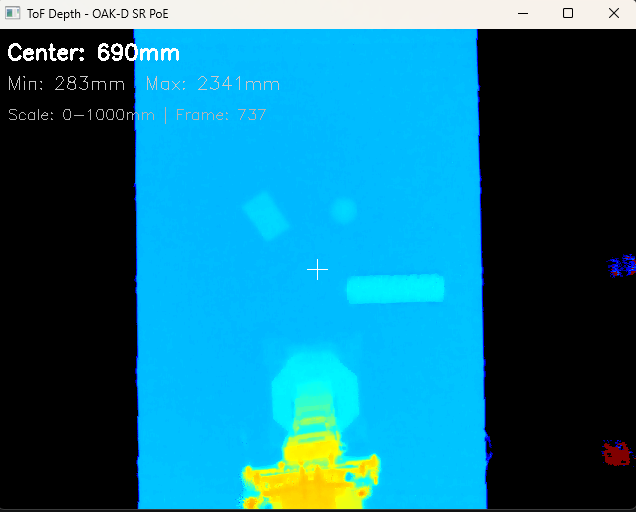
\includegraphics[width=\linewidth]{real_tof_depth.png}
\caption{Raw ToF depth (jet, $0$--$1000$\,mm).}
\end{subfigure}\hfill
\begin{subfigure}{0.40\textwidth}
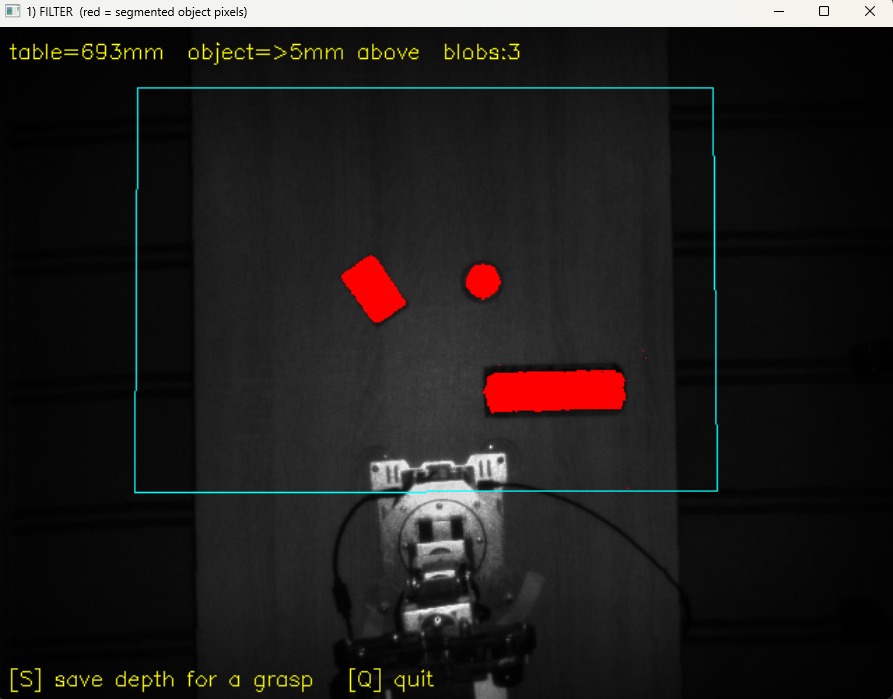
\includegraphics[width=\linewidth]{real_segmentation.png}
\caption{Depth segmentation: table plane at $693$\,mm; above-plane object blobs (red).}
\end{subfigure}
\caption{The physical system through the real overhead OAK-D SR PoE camera. \emph{(a)}~The
raw ToF depth stream (the planar table reads near-uniform; the arm enters from below).
\emph{(b)}~The same median-depth table removal used in simulation, run on the real frame:
the table plane is estimated at $693$\,mm and above-plane object pixels are segmented (red)
for median-centroid extraction.}
\label{fig:realrig}
\end{figure*}

\subsection{Objects}
The same four objects are used in every phase (Table~\ref{tab:objects}). They were chosen
to span a range of grasp difficulty, from a sharp-edged box that the jaws capture easily
to a slim can that nearly fills the gripper. Their grasp-relevant width sets the jaw
capture tolerance as $(55-w)/2$\,mm, where $55$\,mm is the measured real gripper opening.

\begin{table}[t]
\centering
\caption{The four test objects. The jaw capture tolerance is $(55-w)/2$\,mm, where $w$ is
the grasp width and $55$\,mm is the measured real gripper opening.}
\label{tab:objects}
\footnotesize
\resizebox{\columnwidth}{!}{%
\begin{tabular}{lcccl}
\toprule
Object & Width & Height & Jaw tol. & Character \\
       & (mm)  & (mm)   & (mm)     & \\
\midrule
coke\_can  & 52 & 47.3 & 1.5  & largest, fills the jaw \\
banana     & 35 & 26.1 & 10.0 & curved, elongated, 120\,g \\
golf\_ball & 43 & 29.6 & 6.0  & small, round, smooth \\
blue\_box  & 40 & 28.5 & 7.5  & sharp-edged, most robust \\
\bottomrule
\end{tabular}}
\end{table}

\subsection{Conditions}
The core conditions are \texttt{sim\_clean} (noise-free simulated depth),
\texttt{sim\_noisy\_oakd} (the model fitted to the measured OAK-D noise), and
\texttt{sim\_noisy\_nguyen} (the literature model). On top of these, the axial noise term
is swept with \texttt{axial\_scale}~$\in\{1,2,5,10,20\}$, where $\times1$ corresponds to
the measured noise and higher factors probe the estimator's robustness.

\subsection{Trials and metrics}
The pose experiment (Phase~3) was re-run on the current models with roughly 435 frames per
condition and 100\% detection. The simulated manipulation experiment (Phase~4A) is a
varied-placement sweep of 480 analytic trials: each object alone at 20 seeded positions and
orientations over the reachable annulus ($r$ from $0.12$ to $0.30$\,m, full yaw,
IK-validated, with the can lying down), crossed with the six noise conditions
($6\times4\times20$), giving $N=20$ per cell. The real perception experiment (Phase~4B)
uses five real scenes, yielding $n=4$ usable detections per object, because in most scenes
one object drifted into the unreliable ToF edge zone. The real manipulation experiment
(Phase~4C) uses all four objects, each at five placements with three repeats, for 60
trials.

The metrics are: translation RMSE and MAE in millimetres against ground truth (simulated
ground truth in simulation, ChArUco-referenced ground truth on the real system); the
analytic \texttt{grasp\_feasible} success rate as a percentage; and, for the real grasp,
lift-and-hold success with Wilson 95\% confidence intervals. Following the BOP convention,
alignment is taken on the visible top surface only \cite{hodan2018bop}; full 6D pose
metrics are not used because the estimator is translation-only. Detection-to-ground-truth
association uses greedy nearest-neighbour matching.

% =====================================================================
